\section{Algoritmo}
\label{algoritmo}

En esta sección se presenta el algoritmo que se ha implementado para el caso de uso que se ha tratado. El algoritmo se puede ver en el flujograma de la figura \ref{fig:flujo_algoritmo}. \\

\begin{figure}[h]
		\centering
        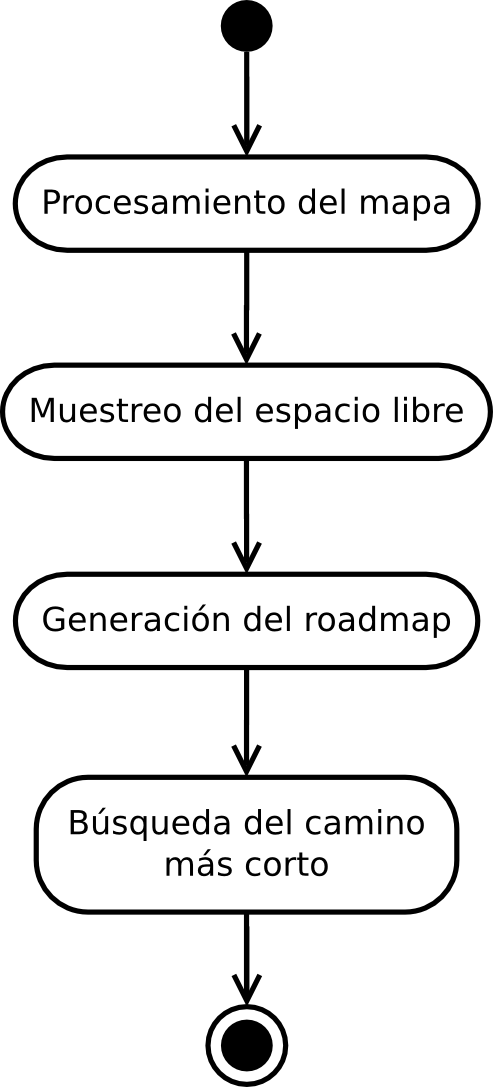
\includegraphics[width=0.2\textwidth]{images/flujo_main.png}
        \caption{Flujograma principal del algoritmo completo}
        \label{fig:flujo_algoritmo}
\end{figure} 


En primer lugar se procesa la imagen obtenida del escenario (mapa) para extraer los obstáculos. A continuación, se generan los puntos (muestras) que corresponderán a los nodos del roadmap y se conectan siguendo un criterio de distancias. Por último, cuando un punto inicial y un punto final son pedidos, se incluyen en el grafo y se calcula el camino más corto mediante un algoritmo de búsqueda en grafos, tal como el Djisktra o el $A^*$.\\

\subsection{Procesamiento del mapa}

A partir de la imagen del escenario capturada desde el simulador, se realiza un procesamiento de la misma usando técnicas de visión por computador. Se comienza por realizar un umbralizado de manera que el resultado es una imagen binaria en la que los obstáculos son píxeles blancos y el espacio libre píxeles negros. \\

A la imagen binaria se le realiza un etiquetado de objetos para obtener los contornos de los distintos obstáculos, los cuales son posteriormente simplificados para reducir el número de puntos que definen el obstáculo, mejorando la eficiencia del algoritmo de detección de colisiones.\\

Estos contornos que definen a los obstáculos son usados en posteriores partes del algoritmo. En la figura \ref{fig:procesado_imagen} se especifica el diagrama de flujo del procesamiento del mapa.\\

\begin{figure}[h]
		\centering
        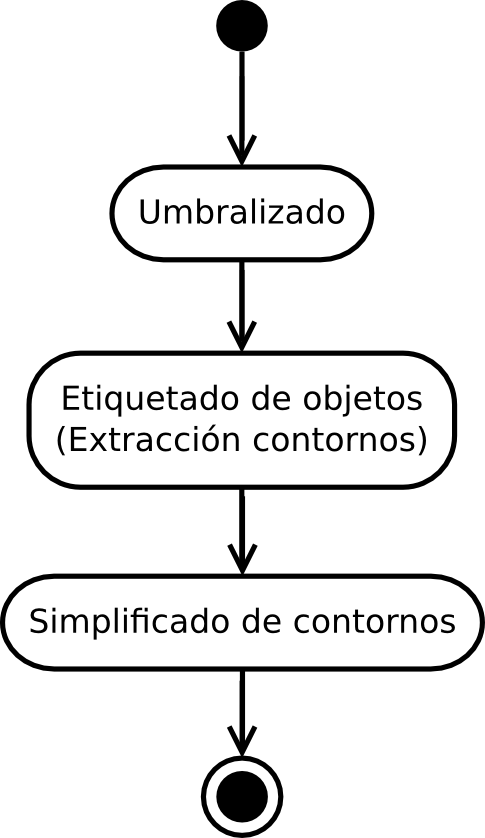
\includegraphics[width=0.2\textwidth]{images/flujo_imagen.png}
        \caption{Flujograma principal del procesamiento del mapa}
        \label{fig:procesado_imagen}
\end{figure} 

\subsection{Muestreo del espacio libre}

El siguiente paso para la generación del roadmap es el muestreo del espacio libre. En el algoritmo original este muestreo se realiza de forma aleatoria, generando nodos del roadmap repartidos aleatoriamente por todo el entorno. La mejora que introduce el artículo que es objeto de estudio con este caso práctico es la generación de dicho muestreo a partir de conjuntos de puntos cuasi-aleatorios. Estas distribuciones de puntos tienen la ventaja de ocupar el espacio libre de forma más eficiente, por lo que con menos cantidad de puntos se puede abarcar un área mayor y, por tanto, más partes delicadas del mapa. Estas partes delicadas pueden ser, por ejemplo, estrechamientos del espacio libre entre obstáculos. Los autores del artículo dan una medida de la ocupación eficiente del espacio libre con un parámetro que ellos llaman \textit{discrepancia}:\\


 \[ D_N(P) = \sup_{j}{\left| \frac{A(J)}{N} -  \mu(J) \right| }\]\\

En la que P es un conjunto de N puntos d-dimensionales, $\left\lbrace x_0, ... , x_{N-1} \right\rbrace$ en $[0,1]^d$, J es cualquier subconjunto rectangular de $[0,1]^d$, $\mu(J)$ es su medida n-dimensional y A(J) es el número de puntos contenido en $P \cap J$.\\

Para el muestreo de puntos cuasi-aleatorios se han usado dos distribuciones de puntos: el conjunto de Hammersley y el conjunto de Halton. Estas distribuciones se generan a partir de una semilla para un número arbitrario de dimensiones. Estas distribuciones se pueden calcular de la siguiente manera:

\subsubsection{Conjunto de Hammersley}

Dados $d-1$ números primos distintos $p_1, p_2, ... , p_{d-1}$ el i-ésimo punto del conjunto es dado por la expresión:

\[ \left( \frac{i}{N}, r_{p_1}(i), ..., r_{p_{d-1}(i)} \right), \qquad i = 0, 1, ..., N-1\]

\subsubsection{Conjunto de Halton}

Dados $d$ números primos distintos $p_1, p_2, ..., p_d$ el i-ésimo punto del conjunto es dado por la siguiente expresión:

\[ \left( r_{p_1}(i),  r_{p_2}(i), ...,  r_{p_d}(i) \right) \]\\~\\

%\subsubsection{Función $r_p(i)$}
En ambos casos, la función $r_p(i)$ se obtiene  escribiendo los dígitos de la notación basada en $p$ en orden inverso. Por ejemplo, para la expresión $i = a_0 + a_1 p + a_2 p^2 + a_3 p^3 + ... $ donde $a_j \in \left\lbrace 0, 1, ... , p-1 \right\rbrace$ la función $r_p(i)$ sería:\\

\[ r_p(i) = \frac{a_0}{p} + \frac{a_1}{p^2} + \frac{a_2}{p^3} + \frac{a_3}{p^4} + ...\]\\


Para nuestra implementación se ha usado una biblioteca ya existente, perteneciente al paquete cgkit que proporciona estos conjuntos de puntos de manera cómoda y rápida, ahorrando tiempo de desarrollo y depuración de errores. La figura \ref{fig:muestreo} muestra una comparativa de los distintos métodos de generación de puntos de muestreo en un escenario ficticio.\\

\begin{figure}[b]
		\centering
        \begin{subfigure}[b]{0.3\textwidth}
                \centering
                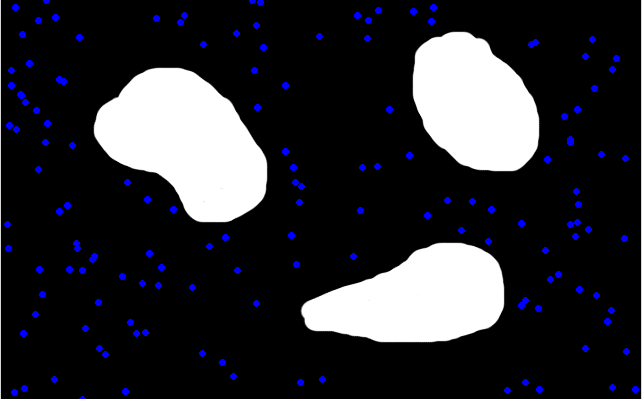
\includegraphics[width=\textwidth]{images/random.png}
                \caption{Muestreo aleatorio}
                \label{fig:muestreo_aleatorio}
        \end{subfigure}
        ~
        \begin{subfigure}[b]{0.3\textwidth}
                \centering
                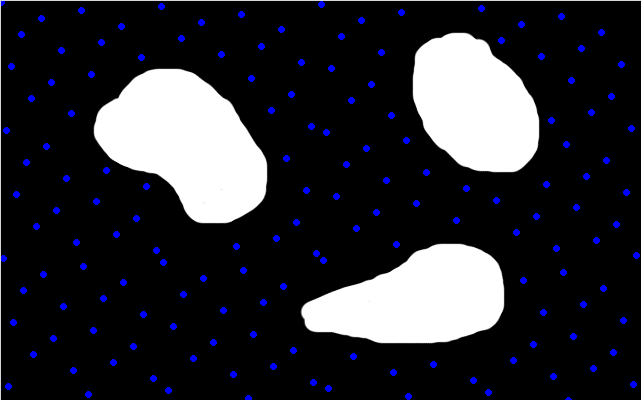
\includegraphics[width=\textwidth]{images/hammersley.png}
                \caption{Muestreo con puntos Hammersley}
                \label{fig:muestreo_hammersley}
        \end{subfigure}
        ~
        \begin{subfigure}[b]{0.3\textwidth}
         	   \centering
                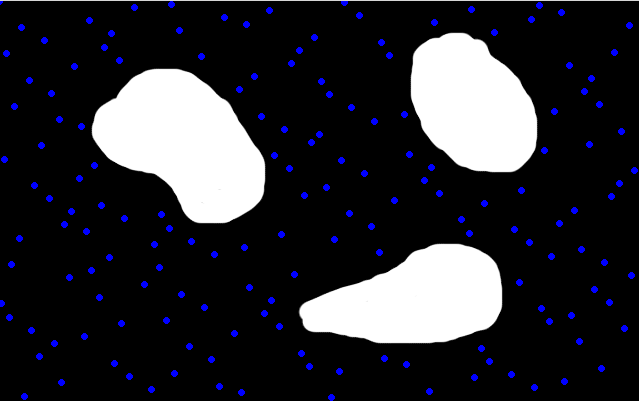
\includegraphics[width=\textwidth]{images/halton.png}
                \caption{Muestreo con puntos Halton}
                \label{fig:muestreo_halton}
        \end{subfigure}
        \caption{Comparativa de los distintos modos de muestreo del espacio libre}\label{fig:muestreo}
\end{figure}

\subsection{Creación del roadmap}
Una vez generados los puntos para el muestreo del espacio libre, se comprueba cada uno de los puntos comprobando colisiones con los obstáculos. Hemos desarrollado tres métodos distintos de comprobación de colisiones para este trabajo:

\begin{itemize}
\item \textbf{Detector de colisiones simple: } Este detector comprueba si el punto se encuentra dentro de alguno de los contornos que definen los obstáculos.
\item \textbf{Detector de colisiones con modelo del robot: } Este detector modela el robot como una circunferencia, y comprueba la colisión entre esta circunferencia y los contornos que definen los obstáculos-
\item \textbf{Detector de colisiones basado en convolución: } Al ser el detector anterior bastante lento en tiempo de cómputo, se aplica primero la convolución del círculo que representa al robot sobre toda la imagen, de forma que los obstáculos se dilatan. De esta forma se puede usar la detección de colisión simple, mucho más rápida, sobre los obstáculos dilatados, combinando las ventajas de los dos enfoques anteriores.
\end{itemize}

Tras eliminar los nodos que colisionan con obstáculos, se prodece a la conexión de los distintos nodos para la generación del grafo del roadmap. El criterio seguido para conectar dos nodos ha sido su vecindad. Se consideran vecinos dos nodos que estén a una distancia entre ellos menor que un valor umbral. Para cada pareja de nodos se calcula la distancia y se coloca en una matriz que reprensenta la conectividad del grafo, y que es usada como entrada de un algoritmo de búsqueda en grafos como Djisktra o $A^*$. Al ser la distancia del nodo A al nodo B la misma que la del nodo B al nodo A, sólo se calculan las distancias una vez.\\

Por último, y antes de añadir cada conexión al roadmap, se comprueba si esa arista del grafo es una trayectoria válida para el robot o colisiona con algún obstáculo, y sólo se añade en caso de que sea válida. Para la comprobación de la arista, se discretiza en diversos puntos, y se comprueba cada uno de ellos con alguno de los métodos presentados anteriormente.\\
